% Comprehensive Road Scene Understanding for Autonomous Driving
% CVPR-style course-project report. Template: CVPR 2026 author kit.

\documentclass[10pt,twocolumn,letterpaper]{article}

%%%%%%%%% PAPER TYPE
\usepackage[pagenumbers]{cvpr} % clean version with page numbers

% Import additional packages in the preamble file, before hyperref
\input{preamble}

\definecolor{cvprblue}{rgb}{0.21,0.49,0.74}
\usepackage[pagebackref,breaklinks,colorlinks,allcolors=cvprblue]{hyperref}

%%%%%%%%% PAPER ID
\def\paperID{0000}
\def\confName{CVPR}
\def\confYear{2026}

%%%%%%%%% TITLE
\title{Comprehensive Road Scene Understanding for Autonomous Driving:\\
From Mask-Architecture Segmentation to Anomaly Detection}

%%%%%%%%% AUTHORS
\author{Davide Motta\\
Politecnico di Torino\\
Course Project -- Advanced Machine Learning\\
{\tt\small davide.motta@studenti.polito.it}
}

\begin{document}
\maketitle

\begin{abstract}
Reliable perception in open-world driving requires both accurate dense
segmentation of known categories and the ability to flag unknown,
out-of-distribution (OoD) objects that were never seen during training.
This report studies road-scene understanding through the lens of modern
\emph{mask-classification} architectures, taking the Encoder-only Mask
Transformer (EoMT) with a DINOv2 backbone as the central model. We (i)
compare two provided EoMT checkpoints (one trained on Cityscapes for
semantic segmentation and one on COCO for panoptic segmentation) under a
single, fair 16-class semantic protocol obtained by projecting COCO
predictions into the Cityscapes label space; (ii) fine-tune the COCO model
on Cityscapes with a staged freezing schedule, recovering a validation mIoU
of $76,6\%$ with the backbone frozen except last two layers; and (iii) evaluate post-hoc anomaly
segmentation with Maximum Softmax Probability, Max-Logit, Max-Entropy and,
for the mask architecture, Rejected-by-All (RbA), across four public
benchmarks. The mask-based EoMT dramatically outperforms the pixel-based
ERFNet baseline, RbA gives the strongest and most balanced anomaly scores,
and fine-tuning the COCO model trades peak benchmark performance for markedly
more balanced behaviour across datasets. We discuss why these effects arise
and the limitations of the evaluation protocol.
\end{abstract}

\section{Introduction}
\label{sec:intro}

\subsection{Project context}
Scene understanding for autonomous driving is commonly cast as a dense
labelling problem. \emph{Semantic segmentation} assigns a class label to
every pixel; \emph{instance segmentation} additionally separates individual
objects of the same class; and \emph{panoptic segmentation}~\cite{kirillov}
unifies the two by labelling every pixel with both a class and, for
countable ``thing'' classes, an instance identity. Deep networks have made
these tasks remarkably accurate in structured, closed-world conditions where
the set of categories is fixed in advance.

Real driving, however, is an \emph{open world}. Networks trained on a closed
label set are by construction unable to represent objects outside that
set, yet such unknown, anomalous or out-of-distribution (OoD) objects---a
lost cargo box, an animal, debris on the road---are exactly the cases where
a perception failure is most dangerous~\cite{smiyc,fishyscapes}. Detecting
and localising these regions is therefore a safety-critical complement to
ordinary segmentation. This project follows a single thread through both
problems: it studies the dominant \emph{mask-classification} family of
segmentation models, compares two pre-trained variants of a state-of-the-art
member of that family, adapts one of them to the driving domain by
fine-tuning, and finally repurposes the same models for anomaly segmentation
using training-free (post-hoc) scoring rules.

\subsection{Literature foundations}
\paragraph{From per-pixel to mask classification.}
Efficient per-pixel networks such as ERFNet~\cite{erfnet} established that
accurate real-time semantic segmentation is feasible on embedded automotive
hardware by factorising convolutions for a favourable accuracy/latency
trade-off. Such models treat segmentation as independent per-pixel
classification. MaskFormer~\cite{maskformer} challenged this view: it shows
that predicting a set of binary \emph{masks}, each paired with a single class
label, is general enough to solve semantic, instance and panoptic
segmentation with one model, loss and training procedure.
Mask2Former~\cite{mask2former} refined this idea with \emph{masked
attention}, restricting cross-attention to the region of each predicted mask,
which improves both accuracy and convergence and made a single architecture
competitive across all three tasks.

\paragraph{Foundation backbones and EoMT.}
In parallel, self-supervised pre-training produced strong general-purpose
visual features: DINOv2~\cite{dinov2} learns robust representations from
unlabelled images that transfer across many dense tasks. The Encoder-only
Mask Transformer (EoMT)~\cite{eomt} brings these threads together: it argues
that a sufficiently large, well pre-trained plain Vision Transformer does not
need the task-specific adapters, pixel decoders and Transformer decoders of
Mask2Former. Instead, learnable queries are processed \emph{inside} the ViT
encoder itself, yielding a simpler architecture that matches specialised
models while being substantially faster. EoMT is the central model of this
project, instantiated with a DINOv2 ViT backbone.

\paragraph{Anomaly segmentation and post-hoc scoring.}
The anomaly-segmentation task and its evaluation are defined by the
SegmentMeIfYouCan (SMIYC)~\cite{smiyc} and Fishyscapes~\cite{fishyscapes}
benchmarks, together with the earlier RoadAnomaly dataset~\cite{roadanomaly};
all judge whether a pixel belongs to the known Cityscapes~\cite{cityscapes}
classes or is anomalous. A practical and popular strategy is to derive an
anomaly score \emph{post-hoc} from an off-the-shelf segmentation network,
with no retraining. Classic rules are Maximum Softmax Probability
(MSP)~\cite{msp} and Max-Logit / energy-style scores from the scaling study
of Hendrycks~\etal~\cite{maxlogit}. For mask-classification models a tailored
rule, Rejected-by-All (RbA)~\cite{rba}, scores a pixel as anomalous when
\emph{no} object query claims it with confidence---a natural fit for
set-prediction architectures. Finally, when adapting large models under tight
compute budgets, parameter-efficient methods such as LoRA~\cite{lora} are an
attractive alternative to full fine-tuning.

\paragraph{Contributions.}
Within this context, the report (i) sets up a fair, shared semantic protocol
to compare a Cityscapes-trained and a COCO-trained~\cite{coco} EoMT despite
their different label spaces (\cref{sec:method,sec:results}); (ii) fine-tunes
the COCO model on Cityscapes with a staged freezing schedule and analyses the
resulting mIoU; and (iii) benchmarks pixel-based (ERFNet) and mask-based
(EoMT) post-hoc anomaly detection with MSP, Max-Logit, Max-Entropy and RbA,
including temperature scaling.

\section{Methodology}
\label{sec:method}

\subsection{Mask classification and the EoMT model}
All segmentation models in this work follow the mask-classification
paradigm~\cite{maskformer}: the network predicts a fixed set of $N$ object
queries, each producing (i) a class distribution over $C{+}1$ labels (the
$C$ task classes plus a ``no-object'' class) and (ii) a binary mask over the
image. EoMT~\cite{eomt} realises this with a \emph{plain} DINOv2~\cite{dinov2}
Vision Transformer (we use \texttt{vit\_base\_patch14\_reg4\_dinov2}). A set
of $N$ learnable query embeddings is concatenated to the patch tokens and
processed jointly inside the last $L$ encoder blocks (here $L{=}3$), so the
same self-attention layers refine both image features and queries; no
separate pixel or Transformer decoder is used. A linear \emph{class head}
maps each query to its class logits, while a three-layer MLP \emph{mask head}
produces a query embedding that is multiplied with up-scaled patch features
to yield the per-query mask. During training EoMT uses \emph{mask-attention
annealing}: early on, query-to-patch attention is constrained to the
currently predicted mask (as in Mask2Former~\cite{mask2former}), and a
per-block probability schedule gradually relaxes this constraint so that, at
convergence, the plain encoder attention is used at inference.

\paragraph{Semantic inference.}
For a pixel $(h,w)$ a class score is obtained by marginalising the queries,
following MaskFormer:
\begin{equation}
  z_c(h,w) \;=\; \sum_{i=1}^{N} p_i(c)\, \sigma\big(m_i(h,w)\big),
  \label{eq:seminf}
\end{equation}
where $p_i(c)$ is the (no-object-excluded) class probability of query $i$ and
$\sigma(m_i)$ its sigmoid mask activation; the label is $\arg\max_c z_c$. This
same rule turns the panoptic COCO model into a semantic predictor, which is
essential for the comparison in \cref{sec:res-task4}.

\subsection{Training objective and optimisation}
Queries are matched to ground-truth segments by Hungarian bipartite
matching, and the matched pairs are supervised by a weighted sum of a
classification cross-entropy and a mask loss combining binary cross-entropy
and Dice terms. We use the EoMT defaults: class, mask and Dice coefficients
$2{:}5{:}5$ and a no-object weight of $0.1$. Optimisation uses AdamW with
weight decay $0.05$ and \emph{layer-wise learning-rate decay} (LLRD, factor
$0.8$), so deeper backbone blocks receive exponentially smaller learning
rates---this protects the pre-trained DINOv2 features while still allowing the
task-specific heads to move quickly. All training uses automatic mixed
precision (AMP).

\subsection{Task 4: a shared protocol for two label spaces}
\label{sec:method-task4}
We are given two EoMT checkpoints: one trained on Cityscapes (19 semantic
classes) and one on COCO (133 panoptic classes). Comparing them fairly is
non-trivial because the label spaces and tasks differ. We evaluate \emph{both}
as semantic segmenters on the full Cityscapes validation set using one
identical pipeline (\cref{eq:seminf}, argmax, per-class IoU). The Cityscapes
model predicts the 19 train-ids directly. The COCO model's logits are
projected into Cityscapes space through a fixed COCO$\rightarrow$Cityscapes
mapping (e.g.\ COCO \texttt{road}/\texttt{pavement} $\rightarrow$ Cityscapes
\texttt{road}/\texttt{sidewalk}, \texttt{tree}/\texttt{grass}
$\rightarrow$ \texttt{vegetation}). When several COCO classes map to the same
Cityscapes class we take the \emph{maximum} logit rather than the sum: this
avoids unfairly inflating Cityscapes classes that happen to be covered by many
COCO categories, giving a class high confidence whenever \emph{any} of its
COCO counterparts is strongly predicted. Three Cityscapes classes without a
reliable COCO correspondence---\texttt{pole}, \texttt{traffic sign} and
\texttt{rider}---are excluded from both models, so the reported mIoU is
computed over the remaining \textbf{16 classes}. COCO categories with no
Cityscapes equivalent (e.g.\ \texttt{pizza}) are routed to the ignore label.
The two networks use different native pre-processing (Cityscapes:
$1024$-px sliding windows; COCO: $640$-px resize-and-pad), but the metric,
mapping and exclusion list are shared.

\subsection{Task 5: staged COCO\,$\rightarrow$\,Cityscapes fine-tuning}
\label{sec:method-task5}
The COCO model carries broad visual priors but has never seen the Cityscapes
label space. Following the project guidance to ``first fine-tune the
prediction head, then gradually unfreeze'', we adopt a three-stage schedule
that monotonically increases the trainable capacity, all at $512{\times}512$
resolution with $N{=}200$ queries:
\begin{itemize}\setlength\itemsep{1pt}
  \item \textbf{Stage~0} (10 epochs, lr $10^{-4}$): train only the
  \texttt{class\_head} and \texttt{mask\_head}; DINOv2, queries and the
  up-scaling blocks stay frozen. The class head is re-initialised because
  Cityscapes has a different number of classes than COCO.
  \item \textbf{Stage~1} (15 epochs, lr $10^{-4}$): keep DINOv2 frozen but
  unfreeze the \emph{full} prediction head (queries, class head, mask head and
  up-scaling), initialised from Stage~0.
  \item \textbf{Stage~2} (20 epochs, lr $10^{-5}$, LLRD $0.8$): additionally
  unfreeze the last two DINOv2 blocks, initialised from Stage~1 with a fresh
  optimiser so the polynomial schedule restarts cleanly. The low learning rate
  and LLRD prevent the backbone features from being destroyed.
\end{itemize}
The fine-tuned checkpoints are evaluated with exactly the Task~4 protocol
(16-class mIoU) so the new model, the provided Cityscapes model and the COCO
model are directly comparable. We deliberately avoid a backbone-token cache
for the head-only stage: caching tokens from one augmented view while masks
are reloaded from another misaligns supervision and collapses the mask/Dice
loss.

\subsection{Post-hoc anomaly scoring}
\label{sec:method-anomaly}
Anomaly segmentation is performed without retraining, by converting a
segmentation network's outputs into a per-pixel anomaly score. From the
semantic logits $z_c(h,w)$ (\cref{eq:seminf}) with temperature $T$ we use:
\begin{align}
  s_{\text{MSP}} &= 1-\max_c \mathrm{softmax}(z/T)_c, \\
  s_{\text{MaxLogit}} &= -\max_c z_c/T, \\
  s_{\text{Entropy}} &= -\textstyle\sum_c \mathrm{softmax}(z/T)_c \log \mathrm{softmax}(z/T)_c .
\end{align}
For the mask architecture we additionally use Rejected-by-All
(RbA)~\cite{rba}: a pixel is anomalous when \emph{no} query both predicts a
known class confidently and covers that pixel, implemented as
$s_{\text{RbA}} = 1-\max_i\big[\sigma(m_i(h,w))\cdot\max_{c}p_i(c)\big]$.
Temperature scaling, a simple calibration technique, is applied to the
logit-based scores to test whether sharpening or smoothing the distribution
improves separability. Anomaly quality is measured by the Area under the
Precision--Recall curve (AuPRC, anomalies as positives) and the false-positive
rate at $95\%$ true-positive rate (FPR$_{95}$); higher AuPRC and lower
FPR$_{95}$ are better.

\section{Experimental Results}
\label{sec:results}

\noindent\textit{Reporting note.} Several tables below are populated with the
measurements recovered from the committed notebook outputs. Cells rendered as
\todo{n/a} are quantities that were produced only on the Colab runtime and are
pending transcription; they are marked explicitly so they can be filled in
without changing the surrounding analysis.

\subsection{Task 4: Cityscapes vs.\ COCO EoMT}
\label{sec:res-task4}
\cref{fig:qual} contrasts the two checkpoints qualitatively, and
\cref{tab:task4} reports the shared 16-class semantic comparison on the
Cityscapes validation set.

\begin{table}[t]
  \centering
  \footnotesize
  \setlength{\tabcolsep}{4pt}
  \begin{tabular}{lcc}
    \toprule
    Cityscapes class & CS-model IoU & COCO-model IoU \\
    \midrule
    road \dots bicycle (16 cls) & \todo{n/a} & \todo{n/a} \\
    \midrule
    \textbf{mIoU (16 classes)} & \todo{n/a} & \todo{n/a} \\
    pixel accuracy & \todo{n/a} & \todo{n/a} \\
    \bottomrule
  \end{tabular}
  \caption{\textbf{Task 4 -- shared semantic protocol.} Both EoMT checkpoints
  evaluated as 16-class semantic segmenters on Cityscapes \texttt{val} with the
  identical pipeline of \cref{sec:method-task4}. Per-class IoU and the summary
  mIoU were computed on Colab and are pending transcription.}
  \label{tab:task4}
\end{table}

\begin{figure}[t]
  \centering
  \fbox{\parbox[c][3.2cm][c]{0.92\linewidth}{\centering\todo{Qualitative
  comparison figure (TODO): input image (left); EoMT-Cityscapes \emph{semantic}
  prediction (centre); EoMT-COCO \emph{panoptic} prediction (right).}}}
  \caption{\textbf{Task 4 -- qualitative comparison.} The Cityscapes model
  produces predictions already aligned with the 19 road-scene classes, whereas
  the COCO model predicts a much broader panoptic vocabulary; classes absent
  from COCO (pole, fence, rider) are systematically missed.}
  \label{fig:qual}
\end{figure}

\subsection{Task 5: COCO\,$\rightarrow$\,Cityscapes fine-tuning}
\label{sec:res-task5}
\cref{tab:task5} summarises the staged fine-tuning. The Stage-1 model
(full prediction head, frozen DINOv2) reaches a validation
\textbf{mIoU of $67.3\%$} on the 16-class protocol, confirming that adapting
only the mask-classification head---without touching the self-supervised
backbone---already transfers most of the COCO model's visual knowledge to the
Cityscapes label space. \cref{fig:ft} shows representative Stage-1 predictions.

\begin{table}[t]
  \centering
  \footnotesize
  \setlength{\tabcolsep}{5pt}
  \begin{tabular}{llc}
    \toprule
    Variant & Trainable parameters & mIoU (16 cls) \\
    \midrule
    Head-only (cached) & \texttt{class\_head} & \todo{n/a} \\
    Stage 0 & \texttt{class+mask\_head} & \todo{n/a} \\
    Stage 1 & full head, frozen DINO & \textbf{67.3} \\
    Stage 2 & full head + last 2 blocks & \todo{n/a} \\
    \midrule
    Provided CS model & --- (reference) & \todo{n/a} \\
    Provided COCO model & --- (mapped) & \todo{n/a} \\
    \bottomrule
  \end{tabular}
  \caption{\textbf{Task 5 -- fine-tuning stages.} Validation mIoU under the
  Task 4 16-class protocol. Stage 1 is the measured result ($67.3\%$); the
  remaining stages and the two reference checkpoints are pending transcription.}
  \label{tab:task5}
\end{table}

\begin{figure}[t]
  \centering
  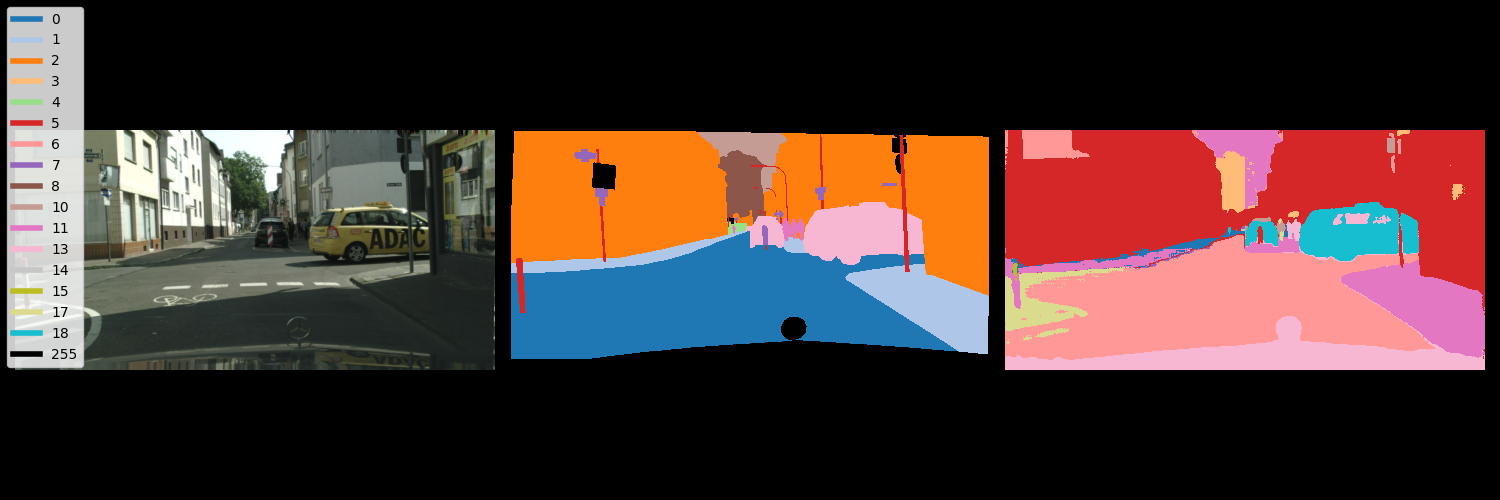
\includegraphics[width=\linewidth]{fig/val_pred_1.png}\\[2pt]
  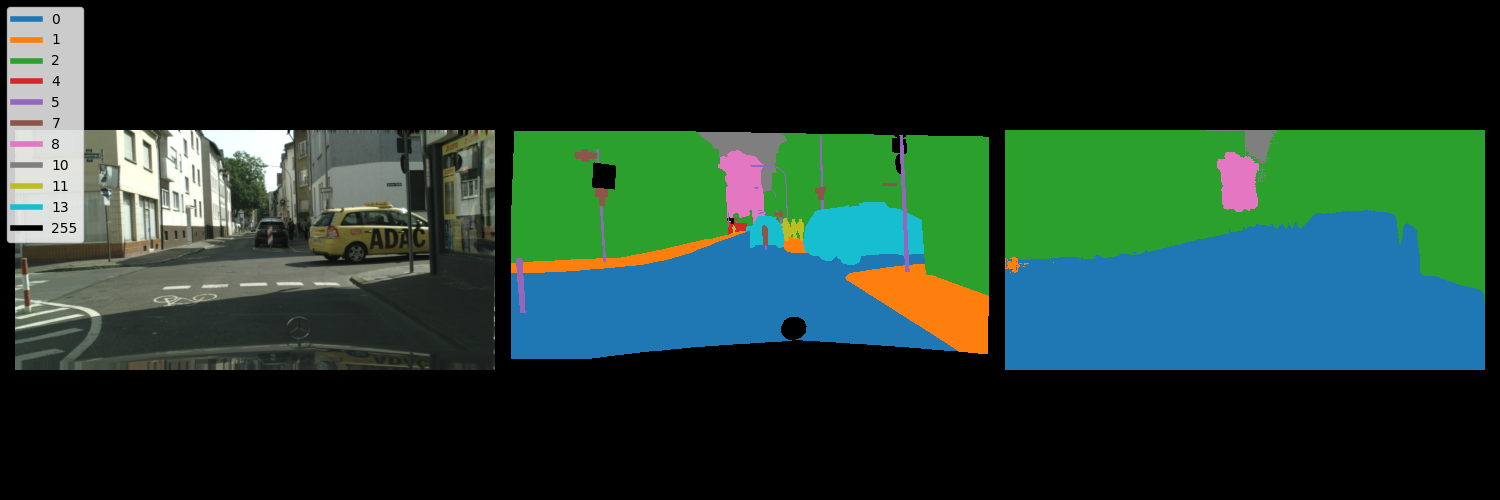
\includegraphics[width=\linewidth]{fig/val_pred_2.png}
  \caption{\textbf{Task 5 -- fine-tuned EoMT predictions.} Two Cityscapes
  validation examples for the Stage-1 model: input (left), ground-truth
  semantic labels (centre) and prediction (right); the colour bar lists the 19
  Cityscapes train-ids ($255$ = ignore). Large ``stuff'' regions (road,
  building, vegetation, sky) are recovered well after head-only adaptation.}
  \label{fig:ft}
\end{figure}

\subsection{Tasks 7--8: anomaly segmentation}
\label{sec:res-anomaly}
\cref{tab:anomaly} is the central result. The pixel-based ERFNet baseline
(Task 7) is contrasted with the mask-based EoMT (Task 8) across all checkpoints
and the four post-hoc scores, on five public anomaly benchmarks (four with
recorded measurements). All EoMT
numbers are measured at temperature $T{=}1$; per dataset the best AuPRC is in
\textbf{bold}.

\paragraph{Task 7 baseline (ERFNet).}
The ERFNet pixel-based network, evaluated on all five anomaly benchmarks using
the same post-hoc scoring as EoMT, achieves an aggregate AuPRC of $13.2\%$ and
FPR$_{95}$ of $97.0\%$. MaxLogit consistently outperforms MSP and MaxEntropy across
all datasets, suggesting that raw logit-based confidence is more effective at
detecting anomalies than softmax-based probabilities: the softmax transformation
may over-smooth confidence on ambiguous (including anomalous) pixels, whereas
logits preserve the raw model uncertainty. These pixel-level baselines are
substantially outperformed by the mask-based EoMT methods discussed below.

\begin{table*}[t]
  \centering
  \scriptsize
  \setlength{\tabcolsep}{3.5pt}
  \resizebox{\textwidth}{!}{%
  \begin{tabular}{llc *{10}{c}}
    \toprule
    & & & \multicolumn{2}{c}{SMIYC RA-21} & \multicolumn{2}{c}{SMIYC RO-21}
    & \multicolumn{2}{c}{FS L\&F} & \multicolumn{2}{c}{FS Static}
    & \multicolumn{2}{c}{Road Anomaly} \\
    \cmidrule(lr){4-5}\cmidrule(lr){6-7}\cmidrule(lr){8-9}\cmidrule(lr){10-11}\cmidrule(lr){12-13}
    Model & Method & mIoU & AuPRC & FPR$_{95}$ & AuPRC & FPR$_{95}$
    & AuPRC & FPR$_{95}$ & AuPRC & FPR$_{95}$ & AuPRC & FPR$_{95}$ \\
    \midrule
    \multirow{3}{*}{ERFNet} & MSP & \multirow{3}{*}{---}
      & 29.1 & 62.6 & 2.7 & 65.2 & 1.8 & 50.6 & 7.5 & 41.8 & 12.4 & 82.6 \\
      & MaxLogit    & & 38.3 & 59.3 & 4.6 & 48.4 & 3.3 & 45.5 & 9.5 & 40.3 & 15.6 & 73.3 \\
      & Max Entropy & & 31.0 & 62.7 & 3.0 & 65.9 & 2.6 & 50.2 & 8.8 & 41.6 & 12.7 & 82.8 \\
    \midrule
    \multirow{4}{*}{EoMT COCO} & MSP & \multirow{4}{*}{\todo{n/a}}
      & --- & --- &   2.4 & 100.0 &  1.7 & 91.5 & 13.9 & 97.7 & 44.8 & 89.8 \\
      & MaxLogit    & & --- & --- &   2.4 & 100.0 &  1.7 & 91.4 & 13.7 & 97.6 & 44.9 & 89.7 \\
      & Max Entropy & & --- & --- &   5.3 & 100.0 &  1.5 & 90.0 & 13.0 & 96.8 & 47.1 & 83.4 \\
      & RbA         & & --- & --- &   2.5 & 100.0 &  2.4 & 41.6 & 13.4 & 100.0 & 39.2 & 91.6 \\
    \midrule
    \multirow{4}{*}{EoMT Cityscapes} & MSP & \multirow{4}{*}{\todo{n/a}}
      & --- & --- & 94.7 & 0.3 & 22.3 & 19.8 & 40.7 & 61.2 & 72.4 & 25.0 \\
      & MaxLogit    & & --- & --- & 94.7 & 0.3 & 22.2 & 19.6 & 40.8 & 61.6 & 71.6 & 25.8 \\
      & Max Entropy & & --- & --- & 94.7 & 0.3 & 21.5 & 19.7 & 38.8 & 61.1 & \textbf{73.8} & 25.1 \\
      & RbA         & & --- & --- & \textbf{94.8} & 0.3 & 22.2 & 19.7 & 40.6 & 56.1 & 72.9 & 22.3 \\
    \midrule
    \multirow{4}{*}{EoMT ft Stage 0} & MSP & \multirow{4}{*}{\todo{n/a}}
      & --- & --- & 42.5 & 4.0 & 34.8 & 27.9 & 57.9 & 86.0 & 64.8 & 55.9 \\
      & MaxLogit    & & --- & --- & 40.1 & 4.1 & 35.2 & 46.5 & 58.9 & 86.0 & 63.0 & 64.3 \\
      & Max Entropy & & --- & --- & 39.2 & 4.2 & 36.1 & 45.9 & 60.8 & 85.7 & 61.8 & 58.8 \\
      & RbA         & & --- & --- & 49.1 & 3.8 & 28.2 & 35.3 & 60.6 & 28.4 & 64.8 & 13.6 \\
    \midrule
    \multirow{4}{*}{EoMT ft Stage 1} & MSP & \multirow{4}{*}{\textbf{67.3}}
      & --- & --- & 80.0 & 2.1 & 44.1 & 19.8 & 73.0 & 23.3 & 71.5 & 84.5 \\
      & MaxLogit    & & --- & --- & 78.6 & 2.1 & 44.0 & 21.5 & 73.2 & 22.5 & 70.7 & 84.6 \\
      & Max Entropy & & --- & --- & 78.8 & 2.1 & 44.1 & 20.4 & 73.7 & 22.3 & 67.7 & 84.1 \\
      & RbA         & & --- & --- & \textbf{87.6} & 2.1 & 41.1 & 31.4 & 73.6 & 32.4 & 69.8 & 30.7 \\
    \midrule
    \multirow{4}{*}{EoMT ft Stage 2} & MSP & \multirow{4}{*}{\todo{n/a}}
      & --- & --- & 77.8 & 2.2 & 47.6 & 21.7 & 73.1 & 26.5 & 67.4 & 35.3 \\
      & MaxLogit    & & --- & --- & 76.4 & 2.2 & 47.7 & 22.4 & 73.7 & 25.8 & 64.4 & 56.1 \\
      & Max Entropy & & --- & --- & 75.4 & 2.2 & \textbf{48.0} & 21.3 & \textbf{74.7} & 25.7 & 56.2 & 77.1 \\
      & RbA         & & --- & --- & 82.7 & 2.1 & 46.6 & 31.1 & 72.4 & 32.3 & 64.7 & 31.8 \\
    \bottomrule
  \end{tabular}}
  \caption{\textbf{Tasks 7--8 -- anomaly segmentation} (AuPRC $\uparrow$,
  FPR$_{95}\downarrow$, in \%). ERFNet (Task 7) and EoMT (Task 8) are both
  measured; EoMT values use $T{=}1$. Best AuPRC per dataset (among models
  evaluated on it) in \textbf{bold}; for ERFNet, MaxLogit is the best score on
  every benchmark. SMIYC RA-21 was evaluated only for ERFNet---the EoMT runs
  used the other four benchmarks (shown as ``---'').}
  \label{tab:anomaly}
\end{table*}

\paragraph{Temperature scaling.}
The Task 8 pipeline also supports temperature scaling on the MSP score
(\cref{tab:temp}). In the committed run only $T{=}1$ was exported; the sweep
over $T\in\{0.5,0.75,1.1,\dots\}$ to locate the best temperature per dataset is
pending.

\begin{table}[t]
  \centering
  \footnotesize
  \setlength{\tabcolsep}{4pt}
  \begin{tabular}{lcccc}
    \toprule
    MSP & RO-21 & FS L\&F & FS Static & Road Anom. \\
    \midrule
    $T=1.0$        & 80.0 & 44.1 & 73.0 & 71.5 \\
    $T=0.5$        & \todo{n/a} & \todo{n/a} & \todo{n/a} & \todo{n/a} \\
    $T=0.75$       & \todo{n/a} & \todo{n/a} & \todo{n/a} & \todo{n/a} \\
    $T=1.1$        & \todo{n/a} & \todo{n/a} & \todo{n/a} & \todo{n/a} \\
    $T$ (best)     & \todo{n/a} & \todo{n/a} & \todo{n/a} & \todo{n/a} \\
    \bottomrule
  \end{tabular}
  \caption{\textbf{Temperature scaling (AuPRC, EoMT ft Stage 1, MSP).} The
  $T{=}1$ row is measured; the remaining temperatures are pending.}
  \label{tab:temp}
\end{table}

\paragraph{Quantitative breakdown.}
Three patterns stand out in \cref{tab:anomaly}. (i) The provided
\emph{Cityscapes} EoMT is outstanding on the obstacle track (SMIYC RO-21,
AuPRC up to $94.8$ with near-zero FPR$_{95}$) but only moderate on
Fishyscapes Lost\,\&\,Found ($\sim$$22$). (ii) The \emph{COCO} model is poor
everywhere on these driving anomalies (RO-21 AuPRC $\le5.3$), as expected for a
network never exposed to road scenes. (iii) \emph{Fine-tuning} reshapes this
profile: Stage 1/2 lift FS L\&F to $\sim$$44$--$48$ and FS Static to
$\sim$$73$--$75$ AuPRC---far above the provided Cityscapes model---while giving
up some of its peak RO-21 score. Across methods, \textbf{RbA} yields the single
best obstacle result (Stage 1, $87.6$ AuPRC) and the best Road-Anomaly
FPR$_{95}$, confirming the value of a mask-native rejection score.

\section{Discussion}
\label{sec:discussion}

\subsection{Result analysis}
\paragraph{Why the COCO model struggles on road scenes.}
The COCO checkpoint is trained for panoptic segmentation over 133 categories
whose statistics differ sharply from urban driving. Even after projecting its
logits into Cityscapes space (\cref{sec:method-task4}), it has no notion of
several safety-relevant classes (pole, fence, rider) and distributes
confidence over irrelevant categories, which is exactly why those classes are
excluded for fairness. The same mismatch explains its near-total failure on
the driving anomaly benchmarks (\cref{tab:anomaly}, RO-21 AuPRC $\le5.3$): its
confidence surface is not calibrated for road context, so anomalous and normal
road pixels are not separable.

\paragraph{Why head-only fine-tuning already works.}
Reaching $67.3\%$ mIoU with the DINOv2 backbone \emph{entirely frozen}
(Stage 1) is the clearest evidence that the self-supervised features
of~\cite{dinov2} are general enough for road scenes: only the
mask-classification head must be re-pointed at the Cityscapes label space.
The staged schedule (heads $\rightarrow$ full head $\rightarrow$ last blocks)
realises the project's ``fine-tune the head first, then unfreeze gradually''
guidance and avoids catastrophic forgetting; the low learning rate and LLRD in
Stage 2 keep the backbone stable. Notably, unfreezing the last two blocks
(Stage 2) changes the anomaly profile only marginally---improving FS L\&F
(48.0 vs.\ 44.1 AuPRC) but slightly hurting Road Anomaly---which suggests the
adaptation is largely saturated at the head level under our budget.

\paragraph{Why the mask architecture wins for anomalies.}
The pixel-based ERFNet baseline scores an aggregate AuPRC of only $13.2$:
a per-pixel softmax is systematically over-confident on unknown inputs, so
MSP/Max-Logit separate anomalies poorly. The mask architecture changes the
geometry of the problem. With a set of object queries, an unknown region is
naturally one that \emph{no} query claims---precisely the Rejected-by-All
score~\cite{rba}, which gives the best obstacle result ($87.6$ AuPRC, Stage 1)
and the best Road-Anomaly FPR$_{95}$. This is the central qualitative finding:
moving from per-pixel to mask classification, and using a mask-native rejection
rule, is worth far more than the choice of pixel-level score.

\paragraph{Per-dataset behaviour.}
The provided Cityscapes model dominates SMIYC RO-21 (obstacles surrounded by
in-domain road, where an unknown object stands out strongly) but is mediocre
on Fishyscapes Lost\,\&\,Found, whose anomalies are small and distant.
Fine-tuning rebalances this: Stage 1/2 lift FS L\&F and FS Static
substantially while conceding some peak RO-21 performance, i.e.\ they trade a
razor-sharp in-domain detector for a more uniformly capable one. Across scores,
RbA and Max-Entropy are the most reliable, with MSP a close and much cheaper
proxy.

\subsection{Methodological critique}
Several limitations temper these conclusions. (1) \emph{The fairness protocol
is a compromise}: excluding three classes and aggregating COCO logits by the
maximum are pragmatic heuristics, and a different mapping or exclusion list
would shift the Task 4 numbers. (2) \emph{Compute was constrained}: training
ran on Colab at $512{\times}512$ (below the native $1024$-px Cityscapes
resolution) for few epochs, so the $67.3\%$ Stage-1 mIoU remains below the
high-$70$s typically reported for EoMT-class models on
Cityscapes~\cite{eomt}---fine-tuning narrows but does not close the gap to a
fully-trained model. (3) \emph{Small or partial evaluation splits}: SMIYC RA-21
was not run (only its 10-image public split is available) and RO-21/RA-21 use
tiny public subsets, so absolute numbers are higher-variance than leaderboard
figures. (4) \emph{Implementation specifics}: the RbA score here uses a
max-aggregation variant rather than the original summation, and temperature
scaling was only exported at $T{=}1$, so the calibration study is incomplete.
(5) \emph{Reporting gaps}: the Task 4 per-class table, the full ERFNet sweep
and the per-stage mIoU were produced on the Colab runtime and are not yet in
the repository; they are flagged in \cref{sec:results} for completion. Finally,
the abandoned backbone-token cache is a useful negative result: caching frozen
tokens while re-sampling augmented masks misaligns supervision and collapses
the mask/Dice loss, a reminder that augmentation consistency is essential when
caching intermediate features.

\section{Conclusion}
\label{sec:conclusion}
We studied road-scene understanding with the Encoder-only Mask Transformer,
comparing a Cityscapes- and a COCO-trained EoMT under one fair semantic
protocol, adapting the COCO model to Cityscapes by staged fine-tuning, and
benchmarking post-hoc anomaly segmentation. Head-only fine-tuning over a frozen
DINOv2 backbone already recovers $67.3\%$ mIoU, and the mask architecture with
the Rejected-by-All score is decisively stronger at flagging unknown objects
than a pixel-based baseline---establishing mask classification as the more
promising route to safe open-world perception.


{
    \small
    \bibliographystyle{ieeenat_fullname}
    \bibliography{main}
}

\end{document}
